\begin{elevator}[Connected Components, and Toplogy]
In this section we introduce some basic notions from topology which will motivate some of our future discussions.
\end{elevator}
\label{hom:sec:connectedcomplex}
It's beyond the scope of this course to define what a topological space is, and the functions between those topological spaces.
The main framework that we'll need is to know the following facts about topological spaces.
\begin{itemize}
    \item Topological spaces are sets with some additional structure (called a topology.)
    \item There are certain functions between these sets, called \emph{continuous functions,} which preserve the useful properties of the topology.
    \item The composition of continuous functions is again continuous. 
    \item If $X$ is a topological space, and $\ZZ_2$ is the topological space with two points, then the set of continuous functions $C^0(X, \ZZ_2)$ is the a vector space. Furthermore, $\dim(C^0(X, \ZZ_2))$ is the number of connected components of $X$. 
\end{itemize}
These are the only properties of topological spaces which we will need to continue this discussion. 
\begin{example}
    The basic example of a topological space is $X:=\RR$. The functions from $f:\RR\to \RR$ which are continuous are exactly the continuous functions you know and love, satisfying the property
    \[\lim_{x_i\to x} f(x_i)=f(x).\]
    This property is fondly phrased as ``when you draw the graph of $f(x)$, there are no jumps in the graph. ''
\end{example}
Some more interesting examples of topological spaces are things like circles, tori, disks, spheres, graphs. 
\[
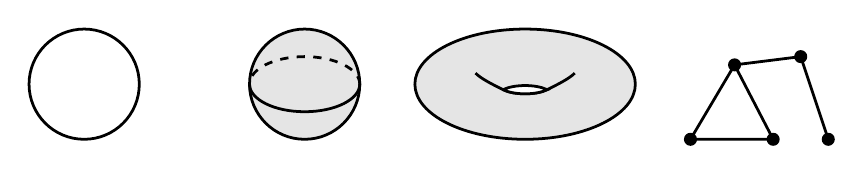
\begin{tikzpicture}[scale=.7]
\newcommand{\vertexradius}{2.5pt}
\newcommand{\vertexscale}{.5}
\newcommand{\bigvertexscale}{1}
\newcommand{\vertex}{\node[circle, fill=black, scale=\vertexscale] }
\newcommand{\highlighta}{red!20}
\newcommand{\highlightb}{blue!20}
\newcommand{\highlightc}{green!20}
\newcommand{\shadinga}{gray!20}
\newcommand{\smallvertex}{\node[circle, fill=black, scale=.2]}
\newcommand{\highlightlinewidth}{3pt}

\tikzset{every path/.style={line width=1 pt}}
    \draw  (-8,1) ellipse (1 and 1);
    \begin{scope}[shift={(2.5,-4)}]
    
    \draw[fill=gray!20]  (-6.5,5) ellipse (1 and 1);
    
    \begin{scope}[]
    \tikzset{every path/.style=};
    \clip  (-8,5) rectangle (-5,4);
    \draw[line width=1pt]  (-6.5,5) ellipse (1 and 0.5);
    \end{scope}
    \begin{scope}[]
    \tikzset{every path/.style=};
    \clip  (-8,6) rectangle (-5,5);
    \draw[dashed, line width=1pt]  (-6.5,5) ellipse (1 and 0.5);
    \end{scope}
    \end{scope}
    \begin{scope}[shift={(2,-4)}]
    \draw[fill=gray!20]  (-2,5) ellipse (2 and 1);
    \draw (-2.9,5.2) .. controls (-2.8,5.1) and (-2.6,5) .. (-2.4,4.9) .. controls (-2.2,4.8) and (-1.8,4.8) .. (-1.6,4.9) .. controls (-1.4,5) and (-1.2,5.1) .. (-1.1,5.2);
    \draw[fill=white] (-2.4,4.9) .. controls (-2.2,5) and (-1.8,5) .. (-1.6,4.9) .. controls (-1.8,4.8) and (-2.2,4.8) .. (-2.4,4.9);
    
    \end{scope}
    
    \begin{scope}[shift={(0.5,0.5)}]
    
    \vertex at (3.3,0.85) {};
    \vertex at (2.5,-0.5) {};
    \vertex at (4,-0.5) {};
    \vertex at (5,-0.5) {};
    \vertex at (4.5,1) {};
    \draw (3.3,0.85) -- (2.5,-0.5) -- (4,-0.5) -- (3.3,0.85) -- (4.5,1) -- (5,-0.5);
    
    \end{scope}\end{tikzpicture}
    \]
Our intuition for continuous maps is that they are the functions between topological spaces which send nearby points to nearby points.
We give a very brief overview of some concepts from topology in \sref{def:topologycc}.

We define the \emph{connected component space of $X$} to be the vector space 
\[C^0(X):=\hom(X, \ZZ_2)\]
of continuous functions from $X$ to the two point set. One can think of this as assigning a color to each connected component of the space $X$, and the number of colorings (determined by the dimension $\dim C^0(X)$) tells you how many connected components there are. 
\[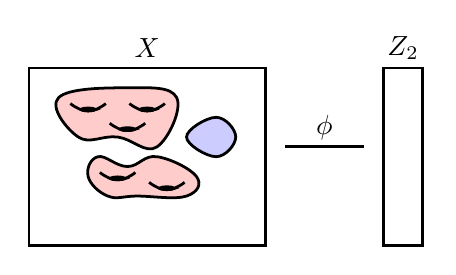
\begin{tikzpicture}[scale=.5]
    \newcommand{\vertexradius}{2.5pt}
\newcommand{\vertexscale}{.5}
\newcommand{\bigvertexscale}{1}
\newcommand{\vertex}{\node[circle, fill=black, scale=\vertexscale] }
\newcommand{\highlighta}{red!20}
\newcommand{\highlightb}{blue!20}
\newcommand{\highlightc}{green!20}
\newcommand{\shadinga}{gray!20}
\newcommand{\smallvertex}{\node[circle, fill=black, scale=.2]}
\newcommand{\highlightlinewidth}{3pt}

\tikzset{every path/.style={line width=1 pt}}
        \begin{scope}[scale=0.5, shift={(-0.5,3)}]
        
        \draw[fill=\highlighta]  plot[smooth cycle, tension=0.7] coordinates {(-4.5,7) (-8,6.5) (-7,4.5) (-5,4.5) (-3,4) (-2,6.5)};
        
        \draw[fill=\highlighta]  plot[smooth cycle, tension=0.7] coordinates {(-6.5,2.5) (-5.5,1.5) (-4,1.5) (-1.5,1.5) (-1,2.5) (-3,3.5) (-4.5,3) (-6,3.5)};
        \draw[fill=\highlightb]  plot[smooth cycle, tension=0.7] coordinates {(-1.5,4.5) (0,3.5) (1,4.5) (0,5.5)};
        
        
        \begin{scope}[shift={(-0.5,-3)}]
        \draw (-2.9,5.2) .. controls (-2.8,5.1) and (-2.6,5) .. (-2.4,4.9) .. controls (-2.2,4.8) and (-1.8,4.8) .. (-1.6,4.9) .. controls (-1.4,5) and (-1.2,5.1) .. (-1.1,5.2);
        \draw[fill=white] (-2.4,4.9) .. controls (-2.2,5) and (-1.8,5) .. (-1.6,4.9) .. controls (-1.8,4.8) and (-2.2,4.8) .. (-2.4,4.9);
        
        \end{scope}
        \begin{scope}[shift={(-3,-2.5)}]
        \draw (-2.9,5.2) .. controls (-2.8,5.1) and (-2.6,5) .. (-2.4,4.9) .. controls (-2.2,4.8) and (-1.8,4.8) .. (-1.6,4.9) .. controls (-1.4,5) and (-1.2,5.1) .. (-1.1,5.2);
        \draw[fill=white] (-2.4,4.9) .. controls (-2.2,5) and (-1.8,5) .. (-1.6,4.9) .. controls (-1.8,4.8) and (-2.2,4.8) .. (-2.4,4.9);
        
        \end{scope}
        \begin{scope}[shift={(-1.5,1)}]
        \draw (-2.9,5.2) .. controls (-2.8,5.1) and (-2.6,5) .. (-2.4,4.9) .. controls (-2.2,4.8) and (-1.8,4.8) .. (-1.6,4.9) .. controls (-1.4,5) and (-1.2,5.1) .. (-1.1,5.2);
        \draw[fill=white] (-2.4,4.9) .. controls (-2.2,5) and (-1.8,5) .. (-1.6,4.9) .. controls (-1.8,4.8) and (-2.2,4.8) .. (-2.4,4.9);
        
        \end{scope}
        \begin{scope}[shift={(-2.5,0)}]
        \draw (-2.9,5.2) .. controls (-2.8,5.1) and (-2.6,5) .. (-2.4,4.9) .. controls (-2.2,4.8) and (-1.8,4.8) .. (-1.6,4.9) .. controls (-1.4,5) and (-1.2,5.1) .. (-1.1,5.2);
        \draw[fill=white] (-2.4,4.9) .. controls (-2.2,5) and (-1.8,5) .. (-1.6,4.9) .. controls (-1.8,4.8) and (-2.2,4.8) .. (-2.4,4.9);
        
        \end{scope}
        \begin{scope}[shift={(-4.5,1)}]
        \draw (-2.9,5.2) .. controls (-2.8,5.1) and (-2.6,5) .. (-2.4,4.9) .. controls (-2.2,4.8) and (-1.8,4.8) .. (-1.6,4.9) .. controls (-1.4,5) and (-1.2,5.1) .. (-1.1,5.2);
        \draw[fill=white] (-2.4,4.9) .. controls (-2.2,5) and (-1.8,5) .. (-1.6,4.9) .. controls (-1.8,4.8) and (-2.2,4.8) .. (-2.4,4.9);
        
        \end{scope}
        \end{scope}
        \vertexa at (4.5,4.5) {};
        \vertexb at (4.5,2) {};
        \draw  (-5,5.5) rectangle (1,1);
        \draw  (4,5.5) rectangle (5,1);
        \draw (1.5,3.5) -- (3.5,3.5);
        \node at (-2,6) {$X$};
        \node at (2.5,4) {$\phi$};
        \node at (4.5,6) {$\mathbb{Z}_2$};
        \end{tikzpicture}\]
    
\begin{claim}[Pullback Map]
    Given a continuous $f: X\to Y$ between topological spaces, there is a map 
    \[f^*: C^0(Y)\to C^0(X).\] 
\end{claim}
\begin{proof}
    The pullback function is defined as before:
    \begin{align*}
        f^*:C^0(Y)\to& C^0(X)\\
        \phi\mapsto& (\phi\circ f)
    \end{align*}
    The only thing to check is that $\phi\circ f$ is a continuous map from $X\to \ZZ_2$; this follows from the composition of continuous maps being continuous. 
\end{proof}
What this claim means is that we can track how the connected components of $X$ are mapped to connected components of $Y$ by using the pullback map.
One interpretation of this is that given a map $f: X\to Y$, we can ``color'' the connected components of $X$ by the connected components of $Y$.

This framework should look very familiar-- it is the same set-up that we used to describe the number of elements in sets.
The connected component space $C^0(X)$ turns questions about connected components into problems in linear algebra instead.
Let us take the annulus, and decompose it into two sets as drawn below. 
This configuration does not respect an inclusion-exclusion like property in the usual sense, in that  $U_1, U_2, X$ each have one connected component, but $U_1\cap U_2$ has two connected components.
\[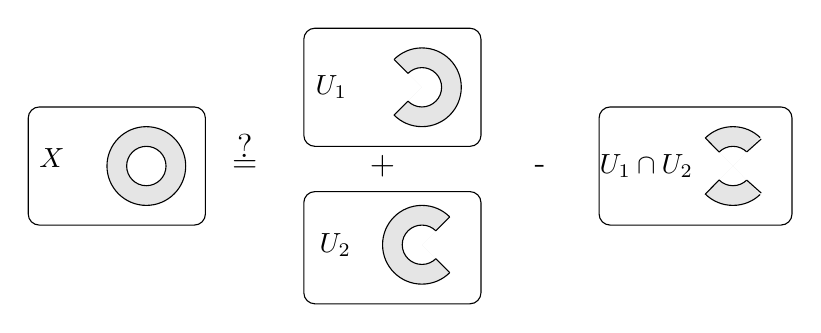
\begin{tikzpicture}[scale=.5]

    \begin{scope}[shift={(-2.5,0)}]
    \draw[rounded corners]  (-5.5,2.5) rectangle (-1,-0.5);
    \draw[fill=gray!20]  (-2.5,1) ellipse (1 and 1);
    \draw[fill=white]  (-2.5,1) ellipse (0.5 and 0.5);
    \node at (-4.9,1.2) {$X$};
    \end{scope}
    
    \begin{scope}[shift={(2,3)}]
    \draw[rounded corners]  (-3,1.5) rectangle (1.5,-1.5);
    \node at (-2.3,0) {$U_1$};\begin{scope}[shift={(2.5,-1)}]
    
    \clip (-2.5,1) -- (-3.65,2.15) -- (-1,2.15) -- (-1,-0.15) -- (-3.65,-0.15) -- cycle;
    \draw[fill=gray!20]  (-2.5,1) ellipse (1 and 1);
    \draw[fill=white]  (-2.5,1) ellipse (0.5 and 0.5);
    \end{scope}
    \draw (135:.5)--(135:1);
    \draw (225:.5)--(225:1);
    \end{scope}
    
    
    \begin{scope}[shift={(9,1)}]
    \draw[rounded corners]  (-2.5,1.5) rectangle (2.4,-1.5);
    \node at (-1.3,0) {$U_1\cap U_2$};\begin{scope}[shift={(3.4,-1)}]
    
    \clip (-2.5,1) -- (-3.65,2.15) -- (-1.4,2.15)-- (-2.5,1) -- (-1.4,-0.15) -- (-3.65,-0.15) -- cycle;
    \draw[fill=gray!20]  (-2.5,1) ellipse (1 and 1);
    \draw[fill=white]  (-2.5,1) ellipse (0.5 and 0.5);
    \end{scope}
    \draw (33:0.6527)--(74:0.7363);
    \draw (-33:0.6527)--(-74:0.7363);
    \draw (16:1.3016)--(23:1.7577);
    \draw (-16:1.3016)--(-23:1.7577);
    \end{scope}
    \begin{scope}[shift={(2,-1)}]
    \draw[rounded corners]  (-3,1.35) rectangle (1.5,-1.5);
    \node at (-2.2,0) {$U_2$};\begin{scope}[shift={(-2.5,-1)}, xscale=-1]
    
    \clip (-2.5,1) -- (-3.65,2.15) -- (-0.5,2) -- (-1,-0.15) -- (-3.65,-0.15) -- cycle;
    \draw[fill=gray!20]  (-2.5,1) ellipse (1 and 1);
    \draw[fill=white]  (-2.5,1) ellipse (0.5 and 0.5);
    \end{scope}
    \draw (45:0.5)--(45:1);
    \draw (-45:0.5)--(-45:1);
    \end{scope}
    \node at (-2.5,1) {\large=};
    \node at (-2.5,1.5) {\large ?};
    \node at (5,1) {\large-};
    \node at (1,1) {\large+};
    \end{tikzpicture}\] 
    
\begin{doubledpage}{example}{Topology 101}{A topological space is a set, equipped with the additional data of \emph{open sets} which determine which points on the topological space are close to each other. In this section, we give a quick overview of point-set topology. }
\label{def:topologycc}
\begin{definition}
    A \emph{topological space} is a pair $(X,\mathcal U)$, where $X$ is a set, and $\mathcal U$ is a specified collection of subsets of $X$, called \emph{open sets} satisfying the following axioms:
    \begin{itemize}
        \item The empty set and whole space $X$ are open sets. 
        \[\emptyset, X\in \mathcal U\]
        \item Any union of open sets is an open set. 
        \[U_\alpha \subset \mathcal U \Rightarrow \left(\bigcup_{\alpha \in A} U_\alpha \right) \in \mathcal U.\]
        \item Any finite intersection of open sets is an open subset. 
        \[\mathcal B\subset \mathcal U , | B|< \infty \Rightarrow \left(\bigcap_{\beta\in B} U_\beta \right) \in \mathcal U.\]
    \end{itemize}
    \end{definition}
    Open sets are kind of strange things. Roughly speaking, if $x$ and $y$ mutually belong to an open set, then we know that they are close to each other in \emph{some} sense, but unlike in the metric space a topology doesn't tell you \emph{how} near two points are two each other. It just tells you that there is something containing both of them. We still get some relative idea of closeness-- if two points mutually belong to many open sets, then we think of them being closer to each other. \\
    Let's introduce a few examples of topologies. 
    \begin{example}[The Discrete Topology]
    Let $X$ be a set. The \emph{discrete topology}  has every subset of $X$ as an open set:
    \[\mathcal U = \{U \;|\; U\subset X\}\]
    This topology has too many open subsets, and all of the points are very far away from each other!
    \end{example}
    A common example of a topological space comes from metric spaces.
    We'll say that a $U$ is open if every point in $x$ is contained within an open ball inside of $U$. 
\newpage
    \begin{example}
    Let $(X, \rho)$ be a metric space. Say that a set $U$ is \emph{$\rho$-open} if for every point $x\in U$, there exists an open ball $B_\epsilon(y)$ with 
    \[x\in B_\epsilon(y)\subseteq U.\]
    Then the collection of sets 
    \[\mathcal U = \{U\subset X \;|\; \text{$U$ is $\rho$-open}\}\]
    makes $(X, \mathcal U)$ a topology. For example, on the real numbers every open interval is an example of an open set with this topology. \label{thm:metrictopology} 
    \end{example}

The interesting maps between topological spaces are those which preserve the topological structure. 
\begin{definition}[Continuous Maps]
    Let $f: X\to Y$ be a function, and $U\subset Y$. The \emph{pre-image} of $Y$ is all the elements of $X$ which get mapped to $U$, 
    \[f^{-1}(U):=\{x\in X\;|\; f(x)\in U\}.\]
    A function $f: X\to Y$ is continuous if and only if for every open set $U\subset Y$, the preimage 
    \[f^{-1}(U)\subset X\]
    is an open set of $X$. 
    \end{definition}
    Suppose that $f: X\to Y$ and $g: Y\to Z$ are continuous maps. Then for any $U\in Z$, $(g\circ f)^{-1}(U)$ is again an open set, which shows that the composition of continuous maps is continuous. 

    A topological space is called \emph{disconnected} if $X=U_1\sqcup U_2$, with $U_1, U_2$ nonempty open sets. The \emph{connected components} of a topological space are the smallest nonempty open sets $\{U_i\}$ so that $X=\bigsqcup_{i=1}^k U_i$. We say that in this case that $X$ has $k$-connected components. 
    \begin{theorem}
        Suppose that $X$ has $k$-connected components. Let $\hom(X, \ZZ_2)$ denote the set of linear maps from $X$ to the space with two points. Then
        \[\dim(\hom(X, \ZZ_2))=k.\] 
    \end{theorem}
\end{doubledpage}
Let's see exactly how the argument from that worked in the proof that $|X|-(|U_1|+|U_2|)+(|U_1\cap U_2|)=0$ fails when we now try to understand the number of connected components. 
The spaces $U_1, U_2, X$ all have one connected component, so 
\[C^0(X)=C^0(U_1)=C^0(U_2)=\ZZ_2.\]
On the other hand, $U_1\cap U_2$ has two connected components, so $C^0(U_1\cap U_2)=\ZZ_2\oplus \ZZ_2$. 
We now look at the inclusions of topological spaces
\[
    \begin{tikzcd}
        U_1\cap U_2 \arrow{r}{i_1} \arrow{d}{i_2} & U_1\arrow{d}{j_1} \\
        U_2\arrow{r}{j_2} & X
          \end{tikzcd}\;\;\;\;\;\;\;
      \begin{tikzcd}
           C^0(U_1\cap U_2 ) &   C^0(U_1) \arrow{l}{i_1^*}\\
           C^0(U_2) \arrow{u}{i_2^*} &  C^0(X) \arrow{u}{j_1^*} \arrow{l}{j_2^*}
      \end{tikzcd}\;\;\;\;\;\;\;
      \begin{tikzcd}
        \ZZ_2\oplus \ZZ_2 &  \ZZ_2 \arrow{l}{i_1^*}\\
        \ZZ_2 \arrow{u}{i_2^*} & \ZZ_2 \arrow{u}{j_1^*} \arrow{l}{j_2^*}
    \end{tikzcd}.
\]
We then condense this down into a sequence of vector spaces by defining $C^1(X):=C^0(U_1)\oplus C^0(U_2)$, and $C^2(X):= C^0(U_1\cap U_2)$. Similarly, we define the maps 
\begin{align*}
    j^*:=j^*_1\oplus j^*_2: C^0(X)\to C^1(X)\\
    i^*:=i^*_1\oplus i^*_2: C^1(X)\to C^2(X).
\end{align*}
as before to give us a sequence of vector spaces and maps between them. 
\[C^0(X)\xrightarrow{j^*}C^1(X)\xrightarrow{i^*}C^2(X)\]
This entire set-up so far follows the same steps as the inclusion-exclusion set up for sets. 
At this point, we deviate from that example. 
\begin{claim}
    For the maps and sets above, the map $j^*$ is injective and  $\im(j^*)\subset \ker(i^*)$.
\end{claim}
\begin{proof}
    Let $\phi:X\to \ZZ_2$ be any continuous function. Then $j^*(\phi)$ is $(j_1)^*\phi\oplus (j_2)^*\phi$, where $(j_1)^*\phi: U_1\to \ZZ_2$ and $(j_2)^*\phi:U_2\to\ZZ_2$ are the restriction of $\phi$ to the subsets $U_1, U_2$. 
    Then 
    \begin{align*}
        (i^*\circ j^*)\phi=(i^*_1\circ j^*_1)\phi+(i^*_2\circ j^*_2)\phi\\
        \intertext{Since $i^*_1j^*_1=i^*_2j^*_2$,}
        =2(i^*_1\circ j^*_1)\phi=0.
    \end{align*}
    This proves that $i^*\circ j^*=0$, which is equivalent to $\im(j^*)\subset \ker(i^*)$. 
\end{proof}
This claim is weaker than the statement that we had for the complex involving sizes of sets. That claim stated that $\im(j^*)=\ker(j^*)$, instead of only having an inclusion, and that $i^*$ was a surjection. 
The discrepancy between these two statements -- equality of image and kernel versus inclusion of image into kernel -- gives us an exact measurement of how the inclusion exclusion principle fails. 